\documentclass[10pt, a5paper]{article}
\usepackage{pdfpages}
\usepackage{parallel}
\usepackage[T2A]{fontenc}
\usepackage{ucs}
\usepackage[utf8x]{inputenc}
\usepackage[polish,english,russian]{babel}
\usepackage{hyperref}
\usepackage{rotating}
\usepackage[inner=2cm,top=1.8cm,outer=2cm,bottom=2.3cm,nohead]{geometry}
\usepackage{listings}
\usepackage{graphicx}
\usepackage{wrapfig}
\usepackage{longtable}
\usepackage{indentfirst}
\usepackage{array}
\newcolumntype{P}[1]{>{\raggedright\arraybackslash}p{#1}}
\frenchspacing
\usepackage{fixltx2e} %text sub- and superscripts
\usepackage{icomma} % коскі ў матэматычным рэжыме
\PreloadUnicodePage{4}

\newcommand{\longpage}{\enlargethispage{\baselineskip}}
\newcommand{\shortpage}{\enlargethispage{-\baselineskip}}

\def\switchlang#1{\expandafter\csname switchlang#1\endcsname}
\def\switchlangbe{
\let\saverefname=\refname%
\def\refname{Літаратура}%
\def\figurename{Іл.}%
}
\def\switchlangen{
\let\saverefname=\refname%
\def\refname{References}%
\def\figurename{Fig.}%
}
\def\switchlangru{
\let\saverefname=\refname%
\let\savefigurename=\figurename%
\def\refname{Литература}%
\def\figurename{Рис.}%
}

\hyphenation{admi-ni-stra-tive}
\hyphenation{ex-pe-ri-ence}
\hyphenation{fle-xi-bi-li-ty}
\hyphenation{Py-thon}
\hyphenation{ma-the-ma-ti-cal}
\hyphenation{re-ported}
\hyphenation{imp-le-menta-tions}
\hyphenation{pro-vides}
\hyphenation{en-gi-neering}
\hyphenation{com-pa-ti-bi-li-ty}
\hyphenation{im-pos-sible}
\hyphenation{desk-top}
\hyphenation{elec-tro-nic}
\hyphenation{com-pa-ny}
\hyphenation{de-ve-lop-ment}
\hyphenation{de-ve-loping}
\hyphenation{de-ve-lop}
\hyphenation{da-ta-ba-se}
\hyphenation{plat-forms}
\hyphenation{or-ga-ni-za-tion}
\hyphenation{pro-gramming}
\hyphenation{in-stru-ments}
\hyphenation{Li-nux}
\hyphenation{sour-ce}
\hyphenation{en-vi-ron-ment}
\hyphenation{Te-le-pathy}
\hyphenation{Li-nux-ov-ka}
\hyphenation{Open-BSD}
\hyphenation{Free-BSD}
\hyphenation{men-ti-on-ed}
\hyphenation{app-li-ca-tion}

\def\progref!#1!{\texttt{#1}}
\renewcommand{\arraystretch}{2} %Іначай формулы ў матрыцы зліпаюцца з лініямі
\usepackage{array}

\def\interview #1 (#2), #3, #4, #5\par{

\section[#1, #3, #4]{#1 -- #3, #4}
\def\qname{LVEE}
\def\aname{#1}
\def\q ##1\par{{\noindent \bf \qname: ##1 }\par}
\def\a{{\noindent \bf \aname: } \def\qname{L}\def\aname{#2}}
}

\def\interview* #1 (#2), #3, #4, #5\par{

\section*{#1\\{\small\rm #3, #4. #5}}

\def\qname{LVEE}
\def\aname{#1}
\def\q ##1\par{{\noindent \bf \qname: ##1 }\par}
\def\a{{\noindent \bf \aname: } \def\qname{L}\def\aname{#2}}
}

\begin{document}
\title{Открытые протоколы --- основа распределенных социальных сетей}
\author{Александр Загацкий\footnote{Витебск, Беларусь, \url{http://zag.ru}, \url{me@zag.ru}}}
\date{}
\maketitle

\begin{abstract}Distributed networks help users to control their online iden\-ti\-ty in the Internet.
Their key feature is absence of a central server. Nodes
in the network belong to each one of its
participants, and software runs on user's computer
or on trusted server. User determines the distribution policy
of his data.
Distributed social networks are built upon open technologies, such as Atom,
Web\-Finder, OpenID/OAuth, Salmon, ActivityStreams and etc.
Most of de\-ve\-loped distributed networks are opensourced and under
development. Some of them are available to use, i.\,e. 
SatausNet "--- the open source microblogging platform that
helps you share and connect in real-time within your own domain. Yet
another distibuted social network OneSocialWeb is a dream of the world where
all social networks are connected and work together similar
to email.
\end{abstract}
Весной этого года в одном из дата-центров провайдера облачного хостинга
Amazon EC2 произошел сбой \cite{zag1}, в результате чего перестали
 функционировать такие сервисы как Friendfeed, Quora, Reddit, Hootsuite,
 Foursquare. По неожиданной случайности это совпало с началом судного дня
 в сериале <<Терминатор: Битва за будущее>>. По сюжету фильма в этот день
 военная компьютерная сеть SkyNet, управляющая военными роботами вышла из
 под контроля человека и произвела ряд ядерных атак на человечество. К
 каким последствиям может привести утрата контроля над персональными
 данными, созданными пользователями в сети и раскрывающие отдельные
 моменты их личной жизни?

 Этот случай заставил задуматься о надежности социальных сервисов и
 сохранности пользовательских данных. Помимо этого за социальными
 сервисами стоят организации. Как следствие, функционирование сервиса
 зависит зачатую от материального положения владельца сервиса. Таким
 образом, сохранность личных данных и контроль над доступом к ним являются
 актуальной задачей для пользователей Интернет.

 Отчасти решить очерченную задачу призваны децентрализованные
 (распределенные) социальные сети. Характерной их особенностью, является
 отсутствие центрального сервера. Узлы сети принадлежат каждому из ее
 участников, а программное обеспечение функционирует на компьютере
 пользователя или на доверенном сервере. При этом пользователь
 самостоятельно определяет политику распространения его данных.

 В основе функционирования распределенных сетей лежат открытые протоколы.
 Ключевыми из них являются следующие:

 \subsubsection*{Atom/RSS}
% \begin{figure}[ht]
%\centering{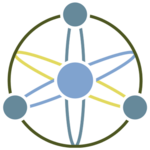
\includegraphics{16_zag1_atom-logo.png}}
%\end{figure}

    Формат синдикации Atom основан на XML и позволяет описывать наборы
    веб-ресурсов. Например: новостные ленты, анонсы статей в блоге,
    галереи фотографий и тому подобное. Формат описан в RFC 4287 \cite{zag2}.

    \subsubsection*{XRD}
 Стандарт описания ресурса доступен в \cite{zag3}. Представляет собой
    последовательное описание данных аккаунта в формате XML. Среди
    данных --- сведения о серверах аутентификации, публичные криптоключи и т.д.

    \subsubsection*{WebFinder}
% \begin{figure}[ht]
%\centering{
\includegraphics{16_zag1_WebFinger.png}}
%\end{figure}
    Протокол, позволяющий идентифицироваться пользователю. В качестве
    идентификации используется запись вида 
    
    \verb!acct:joe@example.com!

    По данному адресу устанавливается сервер с учетной записью
    пользователя и извлекаются XRD-записи.

 \subsubsection*{OpenID/OAuth}
%  \begin{figure}[ht]
%\centering{
\includegraphics{16_zag1_penid-icon.png}}
%\end{figure}
    Протоколы аутентификации и авторизации. Позволяют повысить
    безопасность при взаимодействии нескольких независимых сервисов.

    \subsubsection*{Pubsubhubbub}
%   \begin{figure}[ht]
%\centering{
\includegraphics{16_zag1_pubsubhubbub.png}}
%\end{figure}
    Протокол позволяет сообщать об обновлениях другим ресурсам. При этом
    используются так называемые хабы, которые сообщают об изменениях на
    основном ресурсе подписчикам. Такая схема позволяет реализовать 
    Push-канал обновлений, снизив нагрузку на источник изменений.

    Авторами являются сотрудники Google: Brad Fitzpatrick and Brett
    Slatkin. Источник обновления децентрализуется. Адрес hub для
    обновлений указывается в RSS/Atom в следующем формате:

\noindent     \verb!<link rel="hub" href="http://myhub.example.com/endpoint"/>!


     \subsubsection*{Salmon}
%    \begin{figure}[ht]
%\centering{
\includegraphics{16_zag1_customLogo.png}}
%\end{figure}
    Этот протокол позволяет отправлять действия по отношению к объекту
    (например, статье или заметке) с агрегаторов в оригинальный
    источник. Например, Salmon используется для сбора комментариев к
    оригинальной статье с других сайтов, на которых статья была
    опубликована.

    Адрес для отправки обновлений указан в RSS/Atom:

\noindent        \verb!<link rel="salmon"! \linebreak
\verb!href="http://example.org/salmon-endpoint"/>!

    Особенностью данного протокола является крипто-подпись сообщений,
    которая позволяет решить проблемы со спамом. Для получения
    публичного ключа используется формат XRD.

    \subsubsection*{ActivityStreams}
%    \begin{figure}[ht]
%\centering{
\includegraphics{16_zag1_icon-lg.png}}
%\end{figure}
    Формат описания активности пользователя на ресурсах. Благодаря этому
    формату происходит уведомление узлов распределенной сети о действиях
    пользователей: написании комментария, выставление оценки <<нравится>>,
    публикации фотографий и т.д. Из форматов доступны как JSON, так и
    расширения Atom \cite{zag4}.

    \subsubsection*{XMPP}
    Протокол обмена XMPP (<<Jabber>>) лежит в основе транспорта между
    узлами нескольких распределенных сетей. В качестве клиента
    используется как десктопные программы, так и мобильные версии.

    \subsubsection*{Portable Contacts}
    Протокол безопасного предоставления данных о своих контактах внешним
    сервисам \cite{zag5}. При этом используется протокол OAuth, и
    пользователь управляет доступом к своему списку контактов.

 Среди проектов создания распределенных социальных сетей \linebreak можно отметить
 следующие:
 \begin{description}
	 \item[StatusNet] \cite{zag6}\\
   Открытую платформу для микроблоггинга (аналог Twitter) StatusNet
    можно установить на собственном домене. Платформа предназначена для
    коллективного использования. Лицензия: AGPLv3.
    \item[GNU Social] \cite{zag7}\\
    Соответствует философии Unix: маленькие программы делают маленькие
    работы. По возможностям близка к Status.net: микроблоггинг. Лицензия:
    AGPLv3.
    \item[Diaspora] \cite{zag8}\\
    Проект Diaspora, созданный по инициативе четырех студентов,
    предназначен для персонального использования: ведения микроблога,
    публикации фотографий. Лицензия: AGPL-3.0.
    \item[friendika] \cite{zag9}\\
    Возможности: cервер профилей и поддержка ряда других сетей
    (Diaspora, Google Buzz, Identi.ca, Twitter), поддержка \linebreak шифрования
    между серверами. Лицензия: BSD License.
    \item[OneSocialWeb] \cite{zag10}
    Данная сеть микроблоггинга использует в качестве транспорта протокол
    XMPP \cite{zag11}. В качестве идентификатора пользователя
    используется jabber ID, часть протоколов адаптирована для
    использования в Jabber-сети. Лицензия: Apache 2.
\end{description}
 Это небольшая часть из разрабатываемых проектов, позволяющих
 пользователю сети управлять своими данными и быть независимым в контроле
 над персональной информацией. Тем не менее, очевидно, что персональные
 данные являются основной составляющей социальной жизни в сети и
 определять политику их использования может только пользователь.
\begin{thebibliography}{99}
	\bibitem{zag1} <<Судный день для моих персональных данных>>. \url{http://zag.ru/a4BR2}
	\bibitem{zag2} RFC 4287: The Atom Syndication Format. \url{http://tools.ietf.org/html/rfc4287}
	\bibitem{zag3} Extensible Resource Descriptor (XRD). \url{http://docs.oasis-open.org/xri/xrd/v1.0/xrd-1.0.html}
	\bibitem{zag4} Формат оповещений Activity Streams. \url{http://activitystrea.ms/}
	\bibitem{zag5} Протокол Portable Contacts. \url{http://code.google.com/intl/ru-RU/apis/contacts/docs/poco/1.0/developers_guide.html}
	\bibitem{zag6} Платформа для микроблоггинга StatusNet. \url{http://status.net/}
	\bibitem{zag7} Распределенная сеть GNU Social. \url{http://foocorp.org/projects/social/}
	\bibitem{zag8} Социальная сеть Diaspora. \url{http://www.joindiaspora.com/}
	\bibitem{zag9} Распределенная сеть Friendika. \url{http://project.friendika.com}
	\bibitem{zag10} Социальная сеть OneSocialWeb, построенная на основе протокола XMPP. \url{http://onesocialweb.org/}
	\bibitem{zag11} XMPP "--- открытый протокол обмена сообщениями и информацией о статусе. \url{http://ru.wikipedia.org/wiki/XMPP}
\end{thebibliography}

\end{document}
